  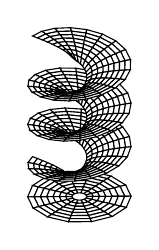
\begin{tikzpicture}

    \begin{axis}[
        axis lines=none,
        axis equal image,
        trig format plots=rad,
        z buffer=sort]
    % log disk
   \addplot3 [
        surf,
        domain=1:7,
        domain y=-pi:pi,
        samples=8,
        samples y=15,
        shader=flat,
        draw=black,
        fill=white
        ]
    ({x*cos(y)},{x*sin(y)},{-12});
    %logspiral
   \addplot3 [
        surf,
        domain=1:7,
        samples=9,
        domain y=-3*pi:3*pi,
        samples y=60,
        shader=flat,
        draw=black,
        fill=white,
        ]
    ({x*cos(y)},{x*sin(y)},{ln(x)+ y});
    \end{axis}
  \end{tikzpicture}%
  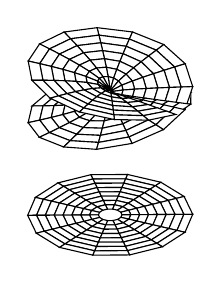
\begin{tikzpicture}
    \begin{axis}[
        axis lines=none,
        axis equal image,
        trig format plots=rad,
        z buffer=sort
        ]
      \addplot3 [
        surf,
        domain=1:7,
        domain y=-pi:pi,
        samples=9,
        samples y=15,
        shader=flat,
        draw=black,
        fill=white
        ]
        ({x*cos(y)},{x*sin(y)},{-12});
      \addplot3 [
        surf,
        domain=0.1:7,
        samples = 8,
        domain y=0:4*pi,
        samples y=30,
        shader=flat,
        draw=black,
        fill=white,
        z buffer=sort
    ] 
    ({x*cos(y)}, {x*sin(y)}, {sqrt(x)*sin(y/2)});
  \end{axis}
  \end{tikzpicture}